%% The first command in your LaTeX source must be the \documentclass command.
%%%% Small single column format, used for CIE, CSUR, DTRAP, JACM, JDIQ, JEA, JERIC, JETC, PACMCGIT, TAAS, TACCESS, TACO, TALG, TALLIP (formerly TALIP), TCPS, TDSCI, TEAC, TECS, TELO, THRI, TIIS, TIOT, TISSEC, TIST, TKDD, TMIS, TOCE, TOCHI, TOCL, TOCS, TOCT, TODAES, TODS, TOIS, TOIT, TOMACS, TOMM (formerly TOMCCAP), TOMPECS, TOMS, TOPC, TOPLAS, TOPS, TOS, TOSEM, TOSN, TQC, TRETS, TSAS, TSC, TSLP, TWEB.
% \documentclass[acmsmall]{acmart}

%%%% Large single column format, used for IMWUT, JOCCH, PACMPL, POMACS, TAP, PACMHCI
% \documentclass[acmlarge,screen]{acmart}

%%%% Large double column format, used for TOG
% \documentclass[acmtog, authorversion]{acmart}

%%%% Generic manuscript mode, required for submission
%%%% and peer review
% \documentclass[manuscript, anonymous, review]{acmart}
\documentclass [sigconf, review, anonymous] {acmart}
\usepackage{todonotes}
\usepackage{xcolor}
\usepackage{subfig}
\usepackage{caption}

%% Fonts used in the template cannot be substituted; margin 
%% adjustments are not allowed.
%%
%% \BibTeX command to typeset BibTeX logo in the docs
\AtBeginDocument{%
  \providecommand\BibTeX{{%
    \normalfont B\kern-0.5em{\scshape i\kern-0.25em b}\kern-0.8em\TeX}}}

%% Rights management information.  This information is sent to you
%% when you complete the rights form.  These commands have SAMPLE
%% values in them; it is your responsibility as an author to replace
%% the commands and values with those provided to you when you
%% complete the rights form.
\setcopyright{acmcopyright}
\copyrightyear{2018}
\acmYear{2018}
\acmDOI{XXXXXXX.XXXXXXX}

%% These commands are for a PROCEEDINGS abstract or paper.
\acmConference[Conference acronym 'XX]{Make sure to enter the correct conference title from your rights confirmation emai}{June 03--05,
  2018}{Woodstock, NY}


\acmBooktitle{Woodstock '18: ACM Symposium on Neural Gaze Detection, June 03--05, 2018, Woodstock, NY} 
\acmPrice{15.00}
\acmISBN{978-1-4503-XXXX-X/18/06}


%%
%% Submission ID.
%% Use this when submitting an article to a sponsored event. You'll
%% receive a unique submission ID from the organizers
%% of the event, and this ID should be used as the parameter to this command.
%%\acmSubmissionID{123-A56-BU3}

%%
%% end of the preamble, start of the body of the document source.
\begin{document}

%%
%% The "title" command has an optional parameter,
%% allowing the author to define a "short title" to be used in page headers.
\title{Empathic Experiences for Shaping Human-Centric Buildings of the Digital Age}

%%
%% The "author" command and its associated commands are used to define
%% the authors and their affiliations.
%% Of note is the shared affiliation of the first two authors, and the
%% "authornote" and "authornotemark" commands
%% used to denote shared contribution to the research.
\author{Shruti Rao}
\email{s.rao@uva.nl}
\orcid{1234-5678-9012}
\affiliation{
  \institution{University of Amsterdam}
  \city{Amsterdam}
  \country{The Netherlands}
}

\author{Hamed Alavi}
\email{h.alavi@uva.nl}
\affiliation{
  \institution{University of Amsterdam}
  \city{Amsterdam}
  \country{The Netherlands}
}

\author{Judith Good}
\email{j.a.good@uva.nl}
\affiliation{
  \institution{University of Amsterdam}
  \city{Amsterdam}
  \country{The Netherlands}
}



%%
%% By default, the full list of authors will be used in the page
%% headers. Often, this list is too long, and will overlap
%% other information printed in the page headers. This command allows
%% the author to define a more concise list
%% of authors' names for this purpose.
\renewcommand{\shortauthors}{Rao et al.}

%%
%% The abstract is a short summary of the work to be presented in the
%% article.
\begin{abstract}
%   Abstracts should be about 150 words.
Given that people spend a significant amount of time within buildings, designing spaces while taking into consideration the impact that they may have on occupants’ well-being is a challenge. While architecture relies on design practices to elicit positive experiences among occupants, they may fall short in terms of sensing occupants and reciprocating their needs in an empathic manner. Therefore, in this position paper, we argue for the need for empathic technologies to shape buildings of the digital age. We believe that buildings that can empathically interact with occupants will enhance occupants’ experiences of well-being in indoor spaces. To that end, we describe one such smart building that may be made human-centric through the incorporation of empathic technologies for various architectural attributes. We thereafter talk of an ongoing case study for identifying the novel, subjective human experiences that may be afforded by empathic buildings of the digital age. 
\end{abstract}

%%
%% The code below is generated by the tool at http://dl.acm.org/ccs.cfm.
%% Please copy and paste the code instead of the example below.
%%

\begin{CCSXML}
<ccs2012>
   <concept>
       <concept_id>10003120</concept_id>
       <concept_desc>Human-centered computing</concept_desc>
       <concept_significance>500</concept_significance>
       </concept>
   <concept>
       <concept_id>10003120.10003123</concept_id>
       <concept_desc>Human-centered computing~Interaction design</concept_desc>
       <concept_significance>500</concept_significance>
       </concept>
   <concept>
       <concept_id>10003120.10003123.10010860</concept_id>
       <concept_desc>Human-centered computing~Interaction design process and methods</concept_desc>
       <concept_significance>300</concept_significance>
       </concept>
   <concept>
       <concept_id>10003120.10003121.10003126</concept_id>
       <concept_desc>Human-centered computing~HCI theory, concepts and models</concept_desc>
       <concept_significance>500</concept_significance>
       </concept>
 </ccs2012>
\end{CCSXML}

\ccsdesc[500]{Human-centered computing}
\ccsdesc[500]{Human-centered computing~Interaction design}
\ccsdesc[300]{Human-centered computing~Interaction design process and methods}
\ccsdesc[500]{Human-centered computing~HCI theory, concepts and models}

%%
%% Keywords. The author(s) should pick words that accurately describe
%% the work being presented. Separate the keywords with commas.
\keywords{affective computing, comfort, smart built environments, hybrid learning spaces, empathic design}

%% A "teaser" image appears between the author and affiliation
%% information and the body of the document, and typically spans the
%% page.
% \begin{teaserfigure}
%   \includegraphics[width=\textwidth]{sampleteaser}
%   \caption{Seattle Mariners at Spring Training, 2010.}
%   \Description{Enjoying the baseball game from the third-base
%   seats. Ichiro Suzuki preparing to bat.}
%   \label{fig:teaser}
% \end{teaserfigure}

 
%%
%% This command processes the author and affiliation and title
%% information and builds the first part of the formatted document.
\maketitle

\section{Introduction}

% Buildings of the Digital Era
Humans are spending a significant amount of time inside increasingly digital buildings \cite{alavi2016future}. Information and communication technologies (ICT) and building energy management systems (BEMS) have resulted in buildings transforming from inanimate structures into interactive and communicative objects \cite{nembrini2017human}. Human occupancy of such spaces results in unfamiliar human-human and human-building interactions whereby buildings now play a more innate role in impacting humans. And although buildings of the digital age can intelligently react to environmental variables such as temperature, light, and air quality \cite{bluyssen2009indoor, moreno2014user}, the buildings' human-centric and empathic behaviour towards occupants remains under-explored. 

% Empathic design for buildings
Human empathy is experienced and conveyed through emotional exchanges based on human experiences. The emotions expressed can take the form of voice and speech patterns, facial expressions, body language, and behavioural patterns \cite{riess2017science}. These cues are recognised by humans, who infer and respond accordingly. Empathy design in Human Computer Interaction (HCI) has therefore focused on developing methods to enable digital technologies to provide ``for the full range of human experience." \cite{wright2008empathy}. With the digitisation of buildings, there is a need to consider them as digital artefacts that too can cater to the full spectrum of human experiences \cite{derix2014empathic}. 

% position
In this position paper, we consider buildings of the digital age that combine architecture with intelligent artefacts. These buildings can enable novel sensory perception of spaces by humans and thereby engender novel human-building interactions. We posit the need for empathic design of buildings that can infer occupants' affective states and interact with occupants in a manner that caters to their subjective experiences in such a way as to improve occupant well-being. 

% paper outline
The remainder of this paper provides a background on architecture in the digital age and the move towards architectural solutions that cater to humans. We then talk about one such smart building and speculate how it can be made empathic. To that end, we describe our case study as a preliminary step towards designing empathic buildings by understanding the needs and experiences of occupants of the smart building. 


\section{Background}
% HBI
Architecture in recent years has begun to question a technologically driven, user-centric design of space at a time when urban densification, sustainability and mental health have become increasing priorities \cite{derix2014empathic}. On the other hand, human-building interaction (HBI) is a burgeoning area of research that focuses on capturing, understanding and enhancing human interactions and experiences both with and within ``smart built environments" \cite{alavi2016future}. The mutual goal of these two fields revolve around understanding,  envisioning and shaping the future of living spaces and all that they encompass \cite{nembrini2017human, alavi2018artifacts}. 

% Examples of work in buildings catering to human needs
In this context, there are several interdisciplinary works that aim to develop human-centric and responsible buildings. For example, smart, sustainable building facades are being developed that adapt to the external environment and react in an energy efficient manner \cite{ahmed2015development}. Other works look at providing comfort to users using responsive materials that react to temperature, light, humidity and air quality \cite{fragkia2020exergy, holstov2015hygromorphic}. These works are often in the form of ``optimally informative" systems such as temperature calendars, air quality forecasts, noise level indicators, and wearables that appropriately inform occupants of their environment and also allow them to engage with comfort parameters to certain degrees  \cite{costanza2016bit, kim2020designing}. Other works take a ``gamified" approach to engage users with their environment and activities in a socially inclusive manner \cite{mathur2015tiny, zhong2022augmenting}. 

% Our perspective
Therefore, much of the work towards developing human-centric buildings focus on changing the environmental variables that may in turn impact the occupants' experiences. Instead, in this position paper, we wish to reconsider the design of human-centric buildings through the perspective of occupant emotions, i.e. empathic buildings that understand and respond to human emotions.


\section{Towards Empathic Experiences in Buildings}
\label{sec:empathic-buildings}
% Why empathic buildings
One significant consequence of smart buildings is the fact that occupants find themselves physically immersed within an interactive object, and therefore experience interactions in a multi-sensory manner \cite{nembrini2017human}. There is therefore the potential for understanding the nature of such interactions, and designing empathic buildings that can infer occupants' emotions and shape the ways in which occupants experience the building. We next discuss how existing buildings can be made empathic from an HCI perspective by identifying three artifacts in an existing smart building.  
 

\subsection{A Digital Building of the Present}
\label{subsec:building}
Our motivation for designing empathic buildings stems from occupying and experiencing a digital building that houses students, researchers, entrepreneurs, and businesses. The building, labelled as an ``intelligent hub", was primarily designed to be human-centric from an architectural standpoint, with a vision to be sustainable, circular and flexible, healthy, and inspiring \footnote{https://link-anonymised-for-blind-review/}. Spaces in the building have been designed to elicit specific human emotions \cite{silo_michiel_2022}. Different artifacts in the interior and exterior have been designed using a variety of materials and design features. The building aims to encourage openness in the lower floors - a glass atrium is used to convey the feeling of transparency to occupants who can view all ongoing activities of the building. A combination of colourful plinth, and display of digital artifacts are used to make occupants feel curious and stimulate collaboration. Quietness and concentration in the upper zones are indicated by specific placement of work spaces, lighting and acoustic treatment. A combination of intelligent sensors throughout the building control light, temperature, and air quality to provide for comfort based on the number of occupants, and external and indoor environmental conditions. However, we question the suitability of relying only on architectural design for invoking emotions and empathy in buildings. 

\begin{figure}[htbp]
\centering
\subfloat[Privacy enabling curtains designed to indicate calm and quiet zones in the middle of corridors. \label{fig:curtain}]{\includegraphics[width=0.23\textwidth]{images/privacy-curtains.jpg}}
\hspace{0.05cm}
\subfloat[Sheer fabric of the curtains questions the privacy-providing aspect.\label{fig:curtain-sheer}] {\includegraphics[width=0.23\textwidth]{images/curtain-sheer.jpg}}

\subfloat[The building staircase designed to encourage users to take the stairs.\label{fig:staircase}]{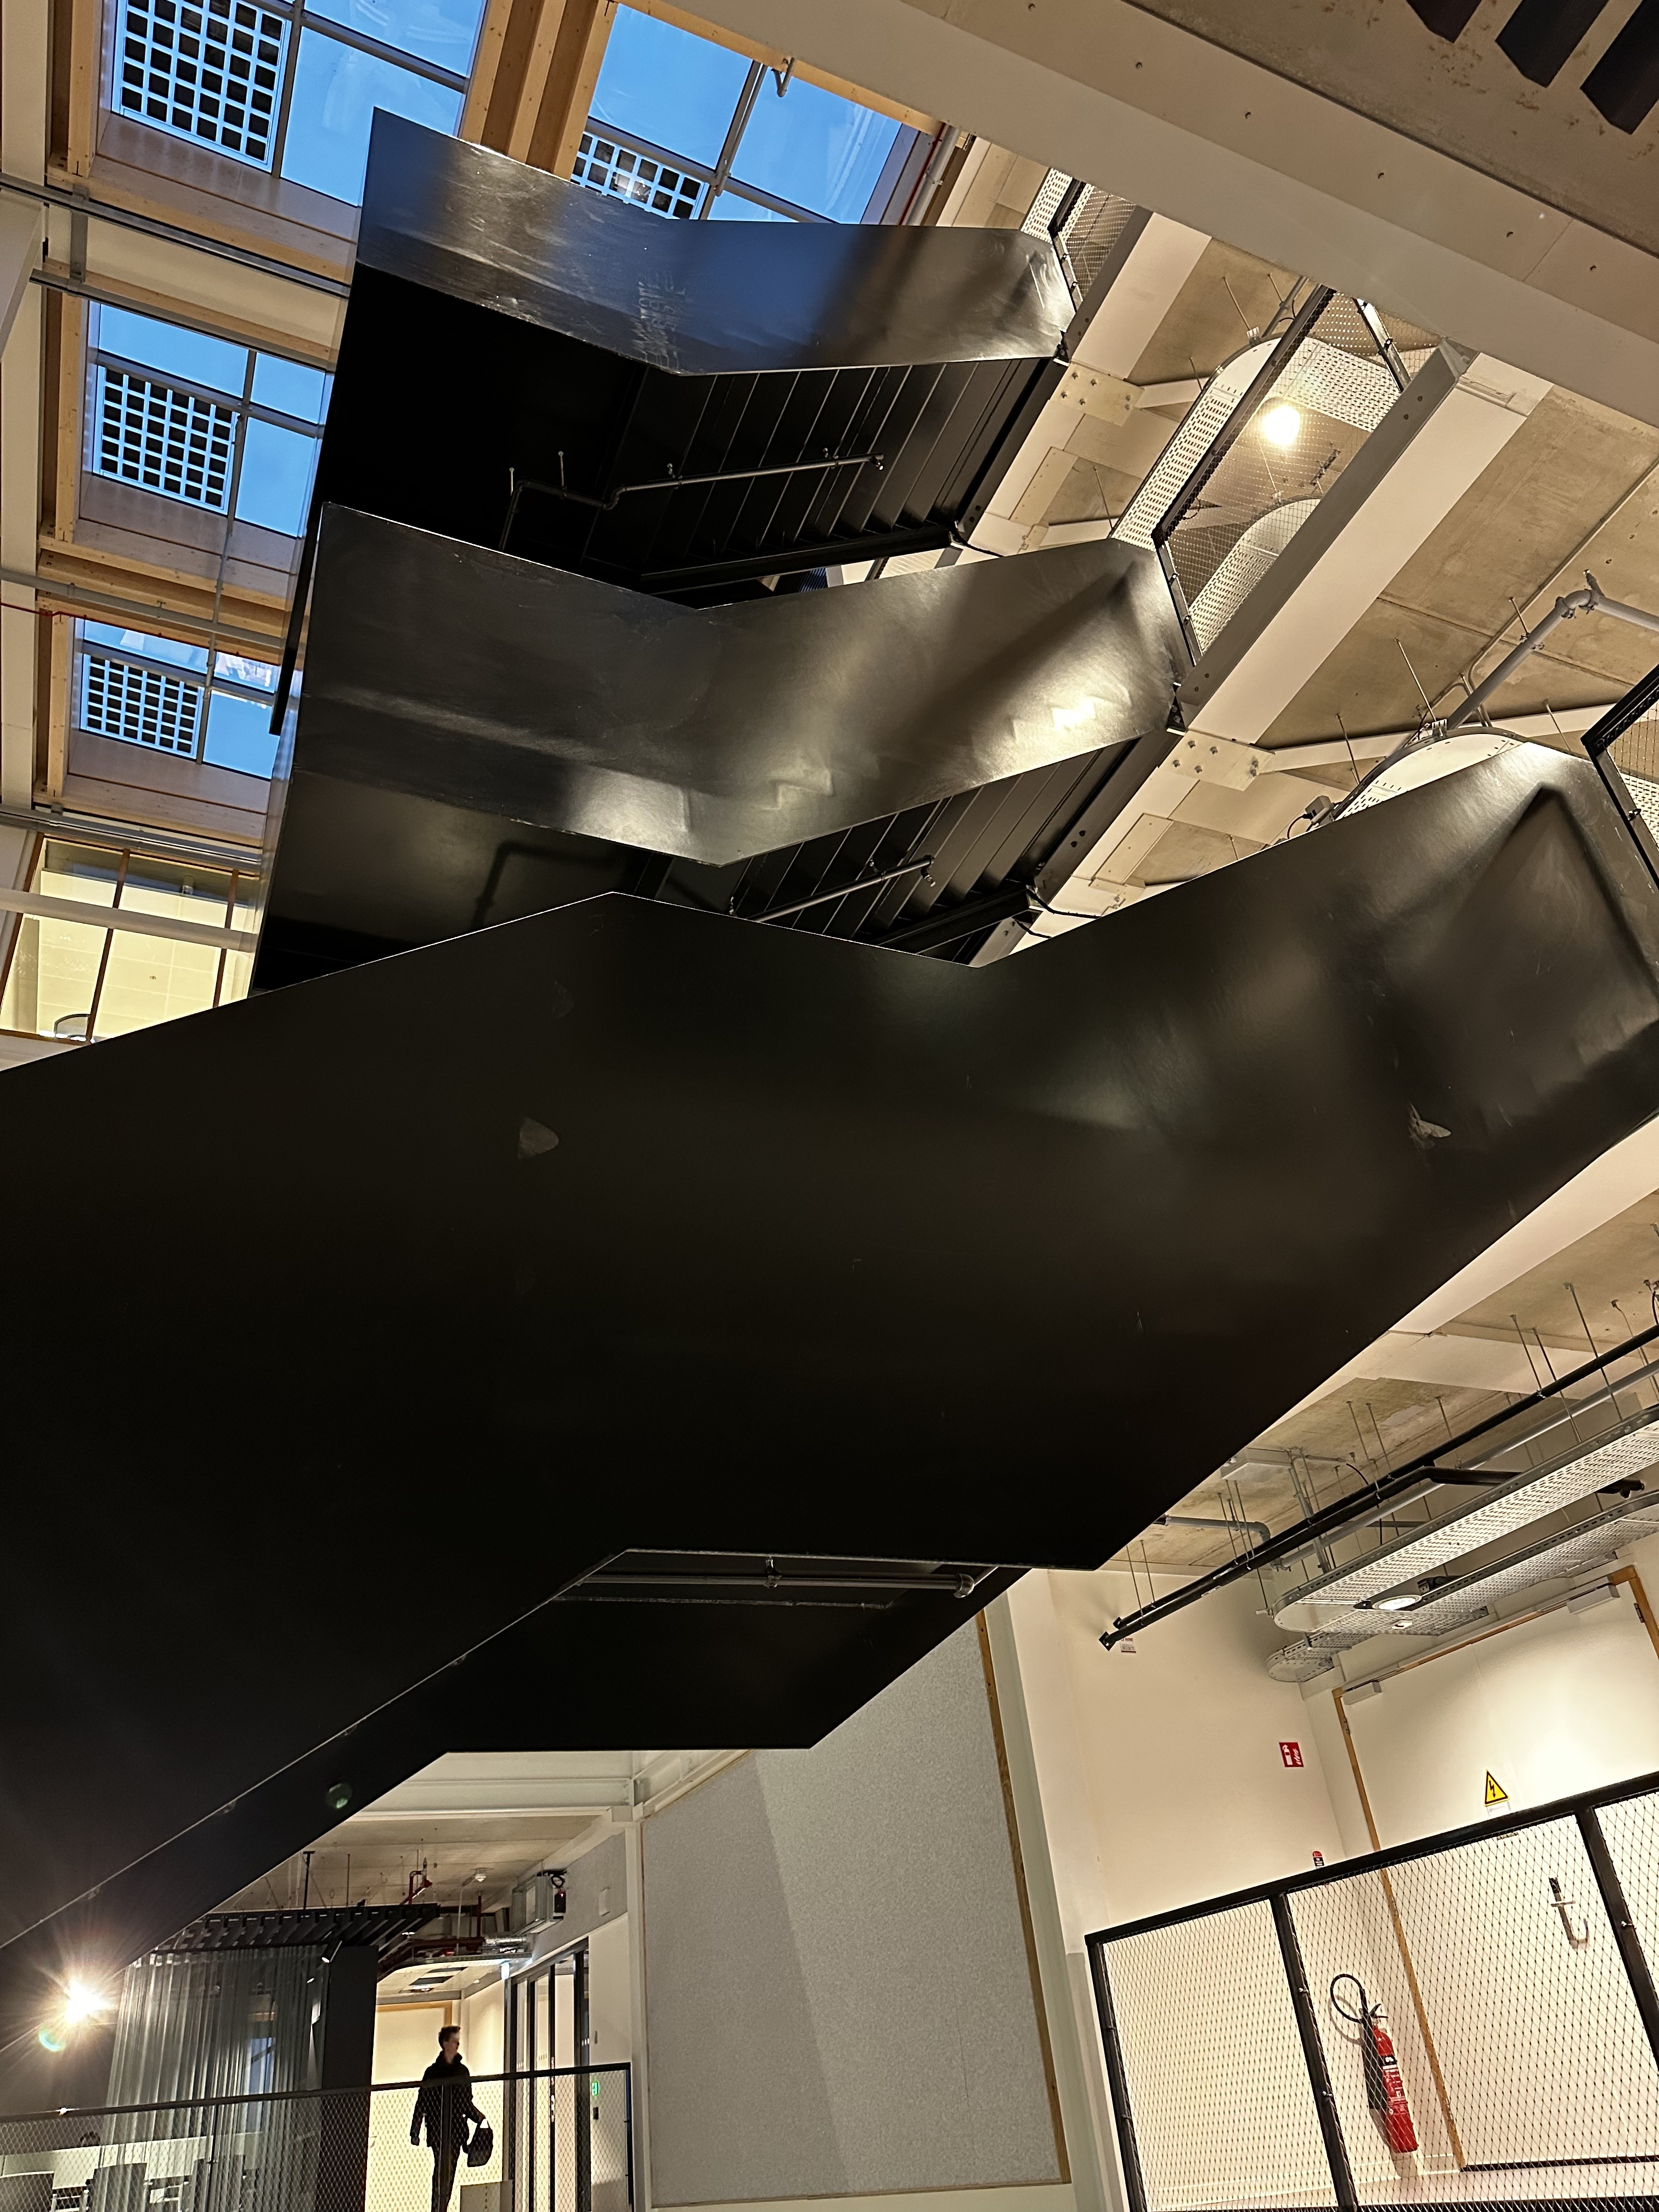
\includegraphics[width=0.23\textwidth]{images/stairs.jpg}}
\hspace{0.05cm}
\subfloat[Material and design features used to incite activity and movement in onlookers \label{fig:staircase-railing}]{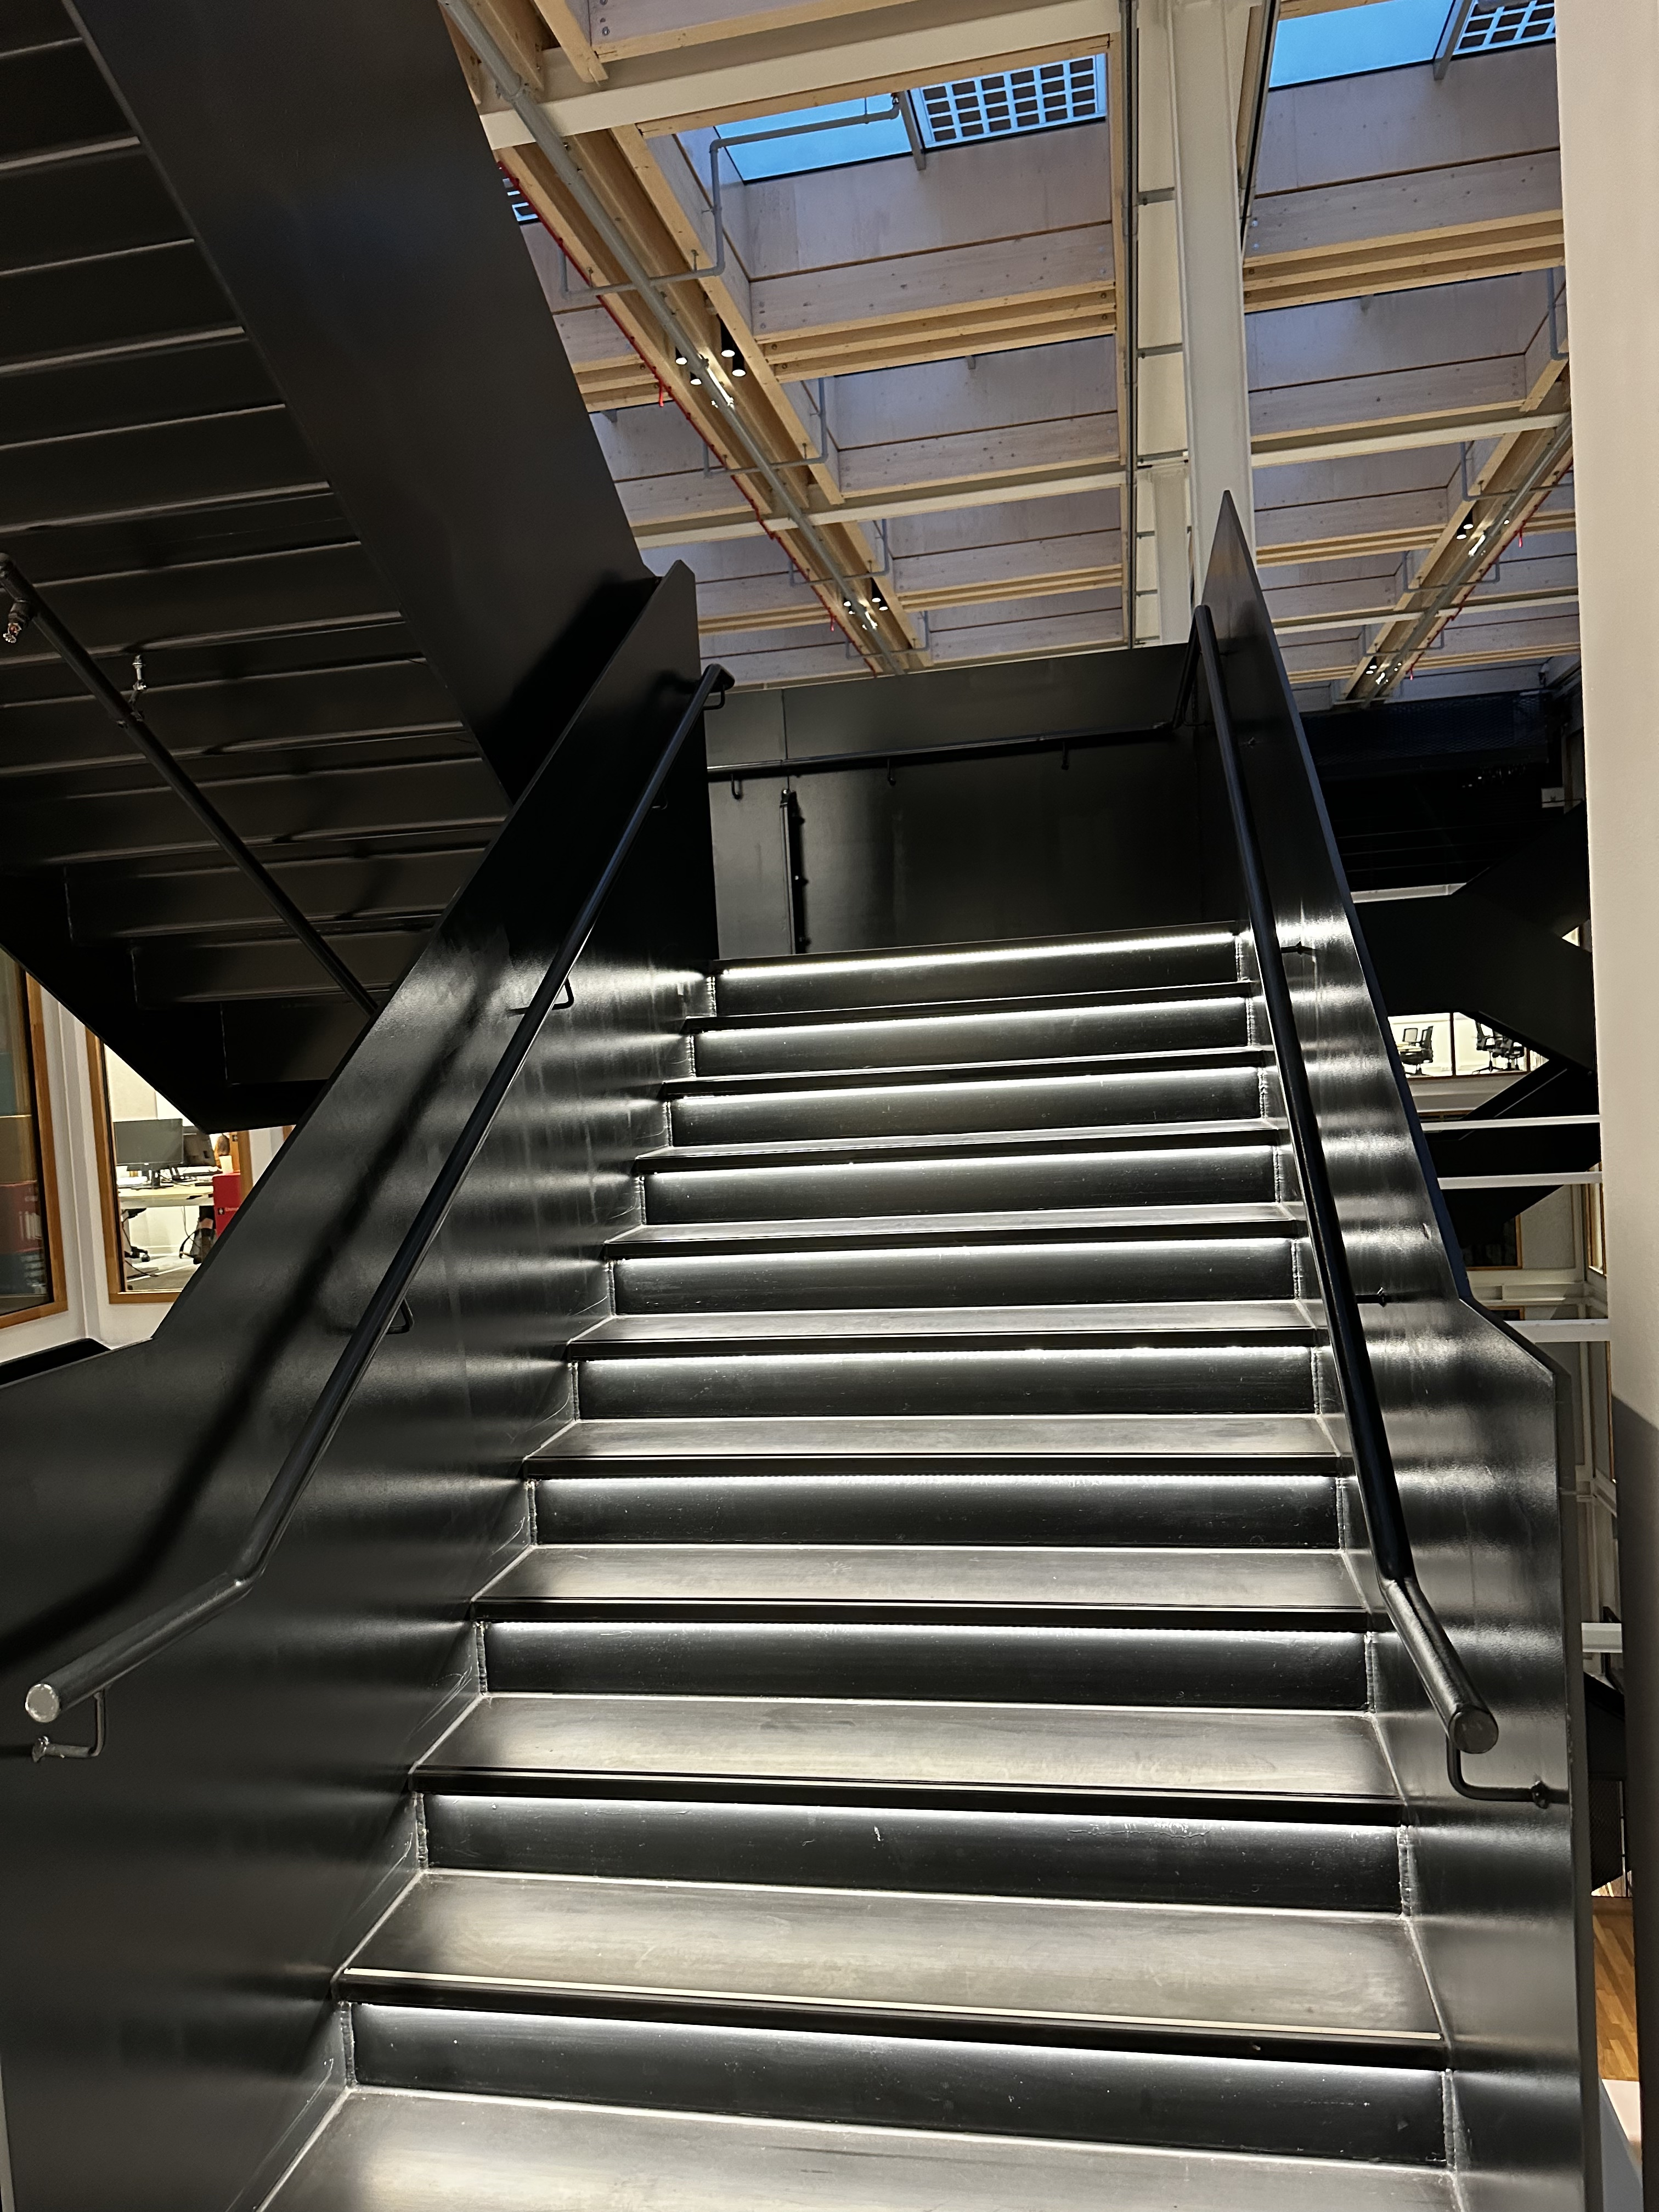
\includegraphics[width=0.23\textwidth]
{images/stairs-closeup.jpg}}

\subfloat[A large screen in the building foyer meant to communicate information about the building with the occupants \label{fig:screen}]
{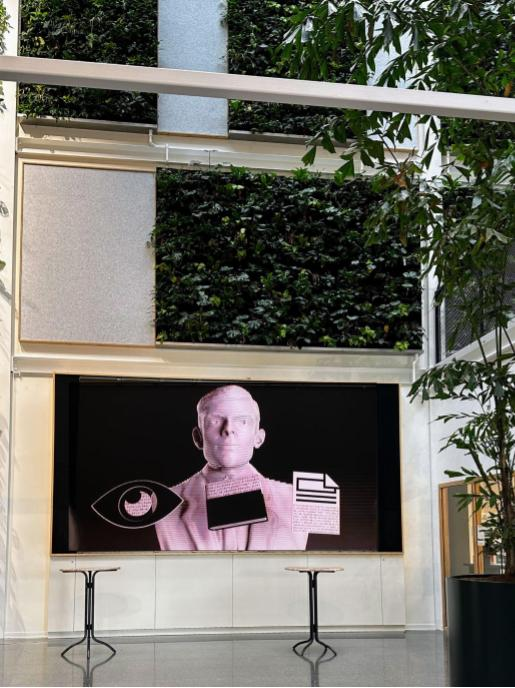
\includegraphics[height=6cm, width=0.3\textwidth]
{images/screen.jpg}}
\caption{Examples of architectural and digital artefacts designed to invoke specific experiences and emotions in the occupants of a smart building} \label{fig:lab42-examples}
\end{figure}

Figure \ref{fig:lab42-examples} shows three tangible artifacts in the building designed to be empathic from an architectural standpoint, but raise questions about the nature of their role in interacting with the building occupants. We speculate on the shortcomings of these artifacts and imagine how intelligent alternatives could be employed towards truly empathic buildings.

\subsubsection*{The Privacy Curtains}
Figures \ref{fig:curtain} and \ref{fig:curtain-sheer} show curtains around certain work spaces in the middle of high-traffic corridors. The curtains serve as a means of providing a sense of privacy and recluse amidst the open and public spaces. However, the sheer material provides transparency and therefore, the clash between privacy and a sheer curtain creates a feeling of confusion and frustration regarding its purpose. An empathic curtain could however intelligently transition between different levels of opacity based on occupants privacy needs (e.g. upon sensing anxiety or distraction).  

\subsubsection*{An Encouraging Staircase}
The building promotes its staircase in Figures \ref{fig:staircase} and \ref{fig:staircase-railing} as being designed to inspire people to climb stairs rather than use the lift (which is tucked away in a corner of the building). However, the design by itself fails to draw occupants to use it - cold and textured wrought iron railings discourages touch and the black, oversized, and floating structure casts a foreboding  shadow on the onlooker,  evoking a feeling of awe - something to observe, rather than use. An empathic staircase that inspires movement could benefit from gamification or anthropomorphisation that, for example, shows calories burnt or muscles exercised as a motivator. 

\subsubsection*{The Digital Interface to the Building}
A large screen in the building foyer accompanied by an interface that allows users to explore and learn different things about the building. The screen may be viewed as a digital building attempting to be transparent and communicate with its occupants. This placement triggers intrigue and a desire to learn more about the building. However, limited information displayed prevents the device from becoming part of an occupant's daily practice (such as the practice of checking one's phone every morning). We envision that a conversational user interface (CUI) may be able to serve as an emphatic medium between the non-digital aspects of the building through a digital means. 

% Our proposed case study
\subsection{Our Proposed Case Study} 
Keeping in mind the need for empathic buildings, we wish to identify artifacts or spaces in buildings where architectural features of empathic design fall short and so could benefit from a more digital design. As a step towards developing such an empathic architecture that can infer occupant emotions, we are undertaking a preliminary case study in the aforementioned building. We first aim to identify occupants' novel and subjective experiences that arise from interactions with and within the smart building. We are particularly interested in understanding occupants' experiences of comfort (based on the indoor environment) and emotions, which is key in built environments \cite{alavi2017comfort}.  We then wish to identify specific influential factors (tangible and intangible) that determine the overall sense of comfort and the emotions experienced in smart building spaces. The case study comprises two phases: (a) emotion and comfort label collection, and (b) a building walk. In the first phase, we will conduct a short survey to obtain a large quantity of occupant derived emotion and comfort information which is grounded in different locations in the building. In the second phase, a building walk will be organised to obtain an in-depth understanding of occupants' perceptions - mental, emotional and physical - towards different spaces in the building.

During the walk, researchers will engage participants in conversations about each space, and conversations will form around what users expect of an empathic building of the future. Questions will investigate different experiential levels (sensory, interpretive, affective and performative) and probe occupants' impressions of the space, usage of space \textit{(Why do you use this space? What kind of tasks would you perform in this space?)}, emotions in the space \textit{(What emotions do you associate with this space?)}, comfort \textit{(Is this space comfortable? Is there sufficient light, warmth, ventilation?)}, shortcomings and scope for improvement. Data collected from both phases will be analysed using both thematic and lexical analysis \cite{braun2006using, xue2020mood}. 


\subsection{Expected Contributions}
We wish to identify where buildings fall short of being understood as empathic and how occupants envision that this could be achieved. Through our case study, we aim to identify specific artifacts (tangible and intangible), as well as the properties of these artifacts that impact the building occupants' emotions. Additionally, we expect to gain an understanding of the lived-in bodily and emotional experiences within smart spaces from a sensory, affective, and interpretive perspective \cite{giaccardi2015foundations}. Our work is a preliminary step towards the design and development of spaces that can understand and respond to the emotional needs of occupants. Results from our findings may be used towards the creation of novel emotion-eliciting experiences that occupants might currently find lacking in smart buildings (e.g. a sense of autonomy and control in an automated building) \cite{moreno2014user}, or enhance certain other experiences (e.g. a feeling of groundedness and familiarity in a space used by many) \cite{rehman2022personalisedcomfort}.  

\section{Conclusion}
The increased complexity of built environments in recent years can be attributed to a growing expectation for buildings to adapt to changing socio-environmental parameters. Given the inevitable transition of buildings into digital spaces, we put forth the need for spaces that cater to the full spectrum of human needs and experiences. In this position paper, we recommend the need for empathic buildings that can understand and respond to occupants' subjective needs. As an alternate to architecturally driven empathic design, we discuss how digital artifacts (tangible and intangible) in smart buildings can be examined, understood and thereby designed for occupants' subjective needs and experiences. To that end, we highlight a case study that will aid in identifying how one such smart building is experienced by its occupants. Our findings may serve as a qualitative first step towards identifying artefacts that may be enhanced through empathic technologies and therefore serve as catalysts for improved human experiences. 

\bibliographystyle{ACM-Reference-Format}
\bibliography{affective-comfort}

\end{document}